\section{Integration management}
\label{sec:integration}
\lhead{\thesection \space Integration Management}
Project Integration Management includes the processes and activities to identify, define, combine, unify, and
coordinate the various processes and project management activities within the Project Management Process
Groups.
\newpage

\subsection{Develop Project Charter}
The created project charter below helps to identify the key information in the project.
All necessary data about the customer and project related risks or issues related to the budget are tackled.

\begin{figure}[!ht]
  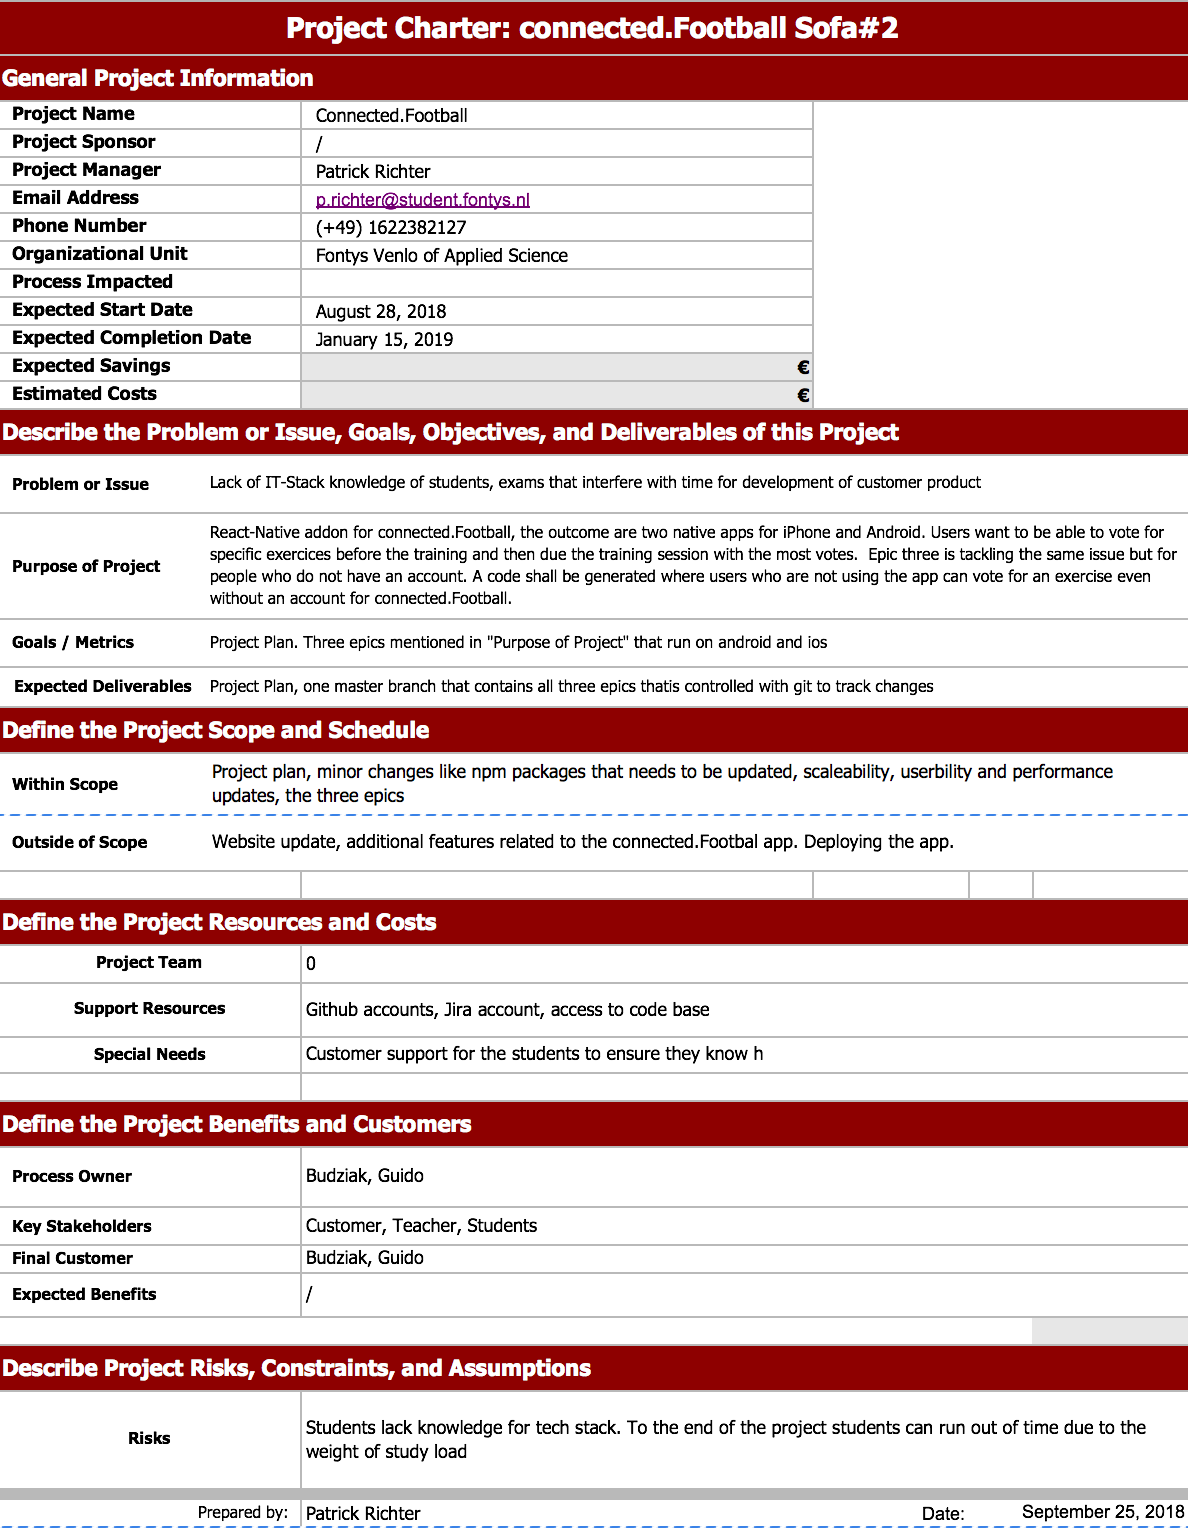
\includegraphics[width=425px, height=585px]{content/diagram/integration/projectChater.png}
  \caption{Project Charter}
\end{figure}
\newpage


\subsection{Perform Integrated Change Control}
A detailed change proposal describes why the change is needed, expected outcomes and impacts, time and resources required, and any other factors that need to be reviewed. 
In this project there is no  change control board (CCB), the project is too small to implement it, so the group decided to skip it. All necessary information and updates are shared directly in the group. Customer related information will be shared in the customer meeting.

\subsection{Close Project or Phase}
At the end of the project, the created Github, Jira and Apple Developer accounts for the students will be returned to the project owner. \newline
After project completion, students will pursue their major and head on to their bachelor thesis.\newline
Besides that, there is no more equipment that has to be returned.

